\section{Introduction}

\begin{definition}[\textit{Integer linear programming problem}]
    An Integer linear programming (ILP) problem is an optimization problem of the form:
    \begin{align*}
        \min                      \:&\: c^Tx           \\
        \text{such that }     &\: Ax = b         \\
                                    &\: x \in \mathbb{Z}^n
    \end{align*}  
\end{definition}
Additionally:
\begin{itemize}
  \item If $x_j \in \left\{ 0, 1 \right\} \: \forall, j$, the problem is called binary linear programming.
  \item If $\exists, i \text{ such that }x_i \notin \mathbb{Z}^n$, then the problem is called mixed integer linear programming.
\end{itemize}
Note that the integrality condition $x_i \in \mathbb{Z}$ is non-linear, as it can be expressed as $\sin(\pi x_j)=0$.
\begin{definition}[\textit{Linear relaxation}]
    Let $ILP$ be an ILP problem:
    \begin{align*}
        z_{ILP}:=\min                      \:&\: c^Tx           \\
        \text{such that }     &\: Ax \leq b               \\
                                    &\: x \in \mathbb{Z}^n      \\
                                    &\: x \leq 0
    \end{align*}  
    Then the Linear Programming (LP) problem:
    \begin{align*}
        z_{LP}:=\max                      \:&\: c^Tx                    \\
        \text{such that }             &\: Ax \leq b               \\
                                            &\: x \leq 0
    \end{align*}  
    is the linear (or continuous) relaxation of $ILP$.
\end{definition}
\begin{property}[Bounds of ILP solutions]  
    For any ILP with $\max$, the optimal solution is bounded by the optimal solution of the LP relaxation:
    \[ z_{ILP} \leq z_{LP} \]
  
    For any ILP with $\min$, the optimal solution is bounded by the optimal solution of the LP relaxation:
    \[ z_{ILP} \geq z_{LP} \]
\end{property}
The feasible region of any ILP is a lattice of points, either finite or infinite, depending on the type of problem.
By removing the integrality constraint, the ILP problem becomes an LP problem, and the optimal solution of the ILP problem isn't always the optimal solution of the LP problem.
\begin{figure}[H]
    \centering
    \begin{subfigure}[b]{0.495\textwidth}
        \centering
        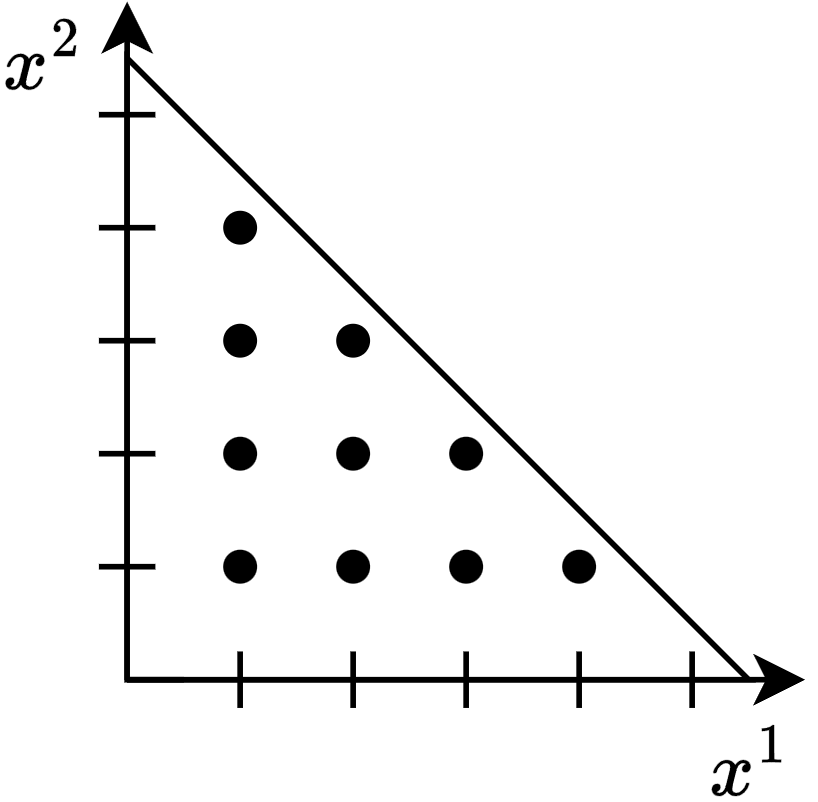
\includegraphics[width=0.4\linewidth]{images/ilp.png}
        \caption{Lattice of integer points}
    \end{subfigure}
    \begin{subfigure}[b]{0.495\textwidth}
        \centering
        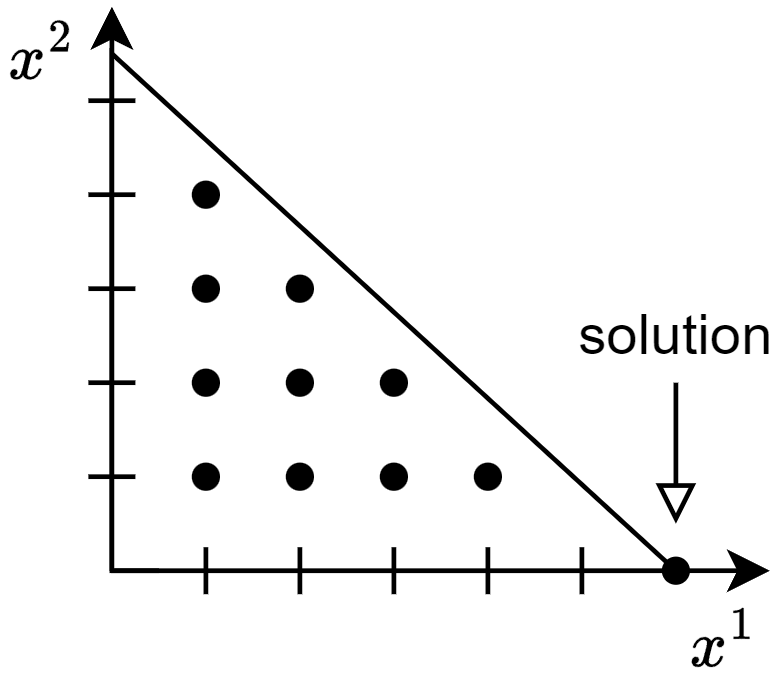
\includegraphics[width=0.4\linewidth]{images/ilp1.png}
        \caption{Relaxed lattice of integer points}
    \end{subfigure}
    \caption{Lattice of integer points}
\end{figure}
  
\subsection{Solutions of the ILP problem}
A viable approach to finding a solution to the ILP problem is to identify a solution to the LP problem and then round it to the nearest integer point.
If an optimal solution of the LP problem is an integer, it is also an optimal solution of the ILP problem. 
However, often the rounded optimal solutions of the LP are either:
\begin{itemize}
    \item \textit{Infeasible} solutions for the ILP.
    \item \textit{Useless} solutions for the ILP, as they are very different from an optimal solution of the ILP.
\end{itemize}
\begin{figure}[H]
    \centering
    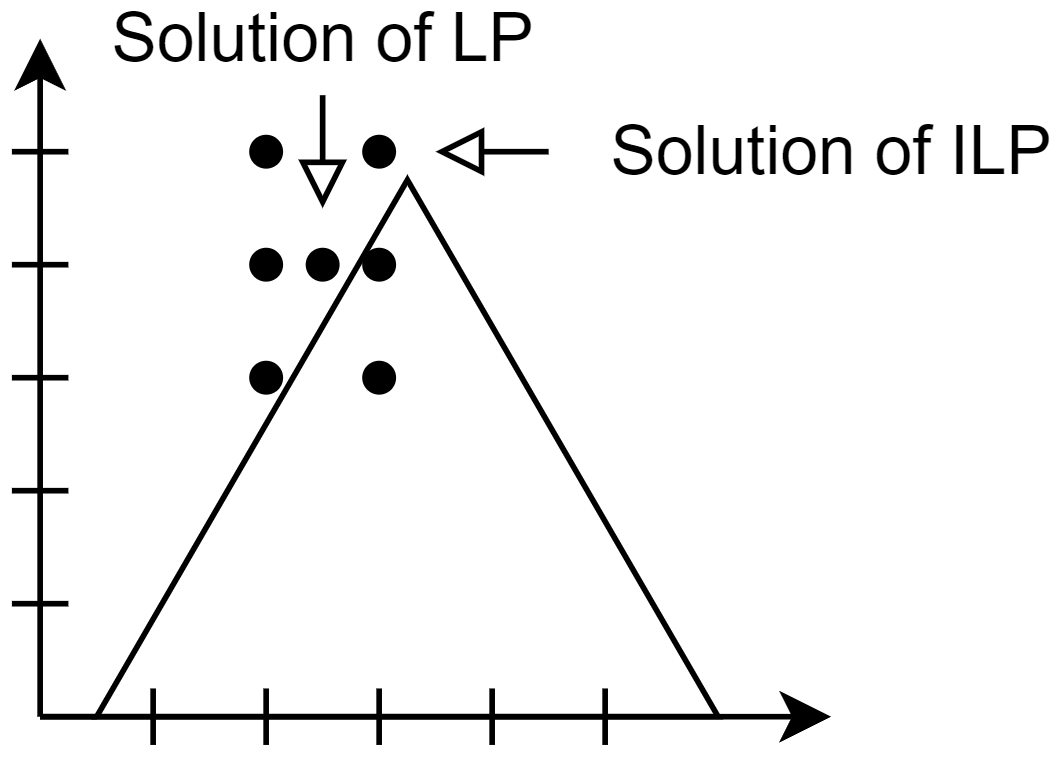
\includegraphics[width=0.25\linewidth]{images/ilp2.png}
    \caption{Solution of the LP relaxation of the ILP problem}
\end{figure}

\subsection{Solution of assignment and transportation problems}
Two crucial ILP problems, namely the assignment and transportation problems, have a solution that is the optimal solution of the LP relaxation.

\paragraph*{Assignment problem}
Given:
\begin{itemize}
    \item $m$ machines, $i = 1, \dots, m$
    \item $n$ jobs, $j = 1, \dots, n$, $n < m$
    \item $c_{ij}$ cost of assigning job $j$ to machine $i$
\end{itemize}
The goal is to determine an assignment of jobs to the machines to minimize the total cost. 
Each job must be assigned to exactly one machine, and each machine should have at least one job. 
The binary variables $x_{ij}$ represent the assignment, where:
\[ x_{ij} = 
\begin{cases}
    1 \quad & \text{if job } j \text{ is assigned to machine } i \\
    0 \quad & \text{otherwise}
\end{cases} \]
The assignment problem can be formulated as the following ILP problem:
\begin{align*}
\min        & \quad \sum_{i=1}^m \sum_{j=1}^n c_{ij} x_{ij}                                                      \\
\text{s.t.} & \quad \sum_{i=1}^{m} x_{ij} = 1 \quad \forall \, j \quad \text{at most one machine for each job}   \\
            & \quad \sum_{j=1}^{n} x_{ij} = 1 \quad \forall \, i  \quad \text{at least one job for each machine} \\
            & \quad x_{ij} \in \left\{ 0, 1 \right\} \quad \forall \, i, j
\end{align*}

\paragraph*{Transportation problem}
Given:
\begin{itemize}
\item $m$ productions plant, $i = 1, \dots, m$.
\item $n$ clients, $j = 1, \dots, n$, $n > m$ by assumption.
\item $c_{ij}$ cost of shipping one unit from plant $i$ to client $j$.
\item $p_i$ production capacity of plant $i$.
\item $d_j$ demand of client $j$.
\item $q_{ij} \geq 0$ quantity shipped from plant $i$ to client $j$.
\end{itemize}
The goal is to determine a transportation plan that minimizes the total costs while satisfying the production and demand constraints. 
The assumption is $\sum_{i=1}^m p_i \geq \sum_{j=1}^{n} d_j$.
Variables $x_{ij}$ represent the quantity shipped from plant $i$ to client $j$.

\paragraph*{Problems analysis}
In the assignment problem example, a forcing constraint is present, while the transportation problem introduces a constraint limiting the active number of variables.
\begin{definition}[\textit{Forcing constraint}]
    A constraint in the form: 
    \[ \displaystyle x \leq y\]
    is termed a forcing constraint if both $x$ and $y$ are binary variables.
\end{definition}
\begin{definition}[\textit{Constraint on binary variables}]
    A constraint of the form:
    \[ \displaystyle \sum_{i=1}^n x_i \leq 1 \]
    where all $x_i$ are binary variables, implies that at most one of the variables $x_i$ can be one. 
    Similarly, a constraint in the form: 
    \[ \displaystyle \sum_{i=1}^n x_i = 1 \]
    where all $x_i$ are binary variables, implies that exactly one variable $x_i$ must be one.
\end{definition}
The transportation problem illustrates that the optimal solution of the LP relaxation of the transportation problem is also the optimal solution of the ILP problem.
\begin{theorem}[Solution of the transportation problem]
    If in a transportation problem $p_i, \ d_{ij}, \ q_{ij}$ are all integers, all the basic feasible solutions (vertices) of its linear relaxation are integers.
\end{theorem}
\begin{proof}
    Let $A$ be an integer constraint matrix of size $\left( mn + n + m \right) \times \left( mn \right)$, where $a_{ij} \in \left\{ -1, 0, 1 \right\}$.
    The right-hand side vector $b$ is composed of integer elements.
    The optimal solution for the linear relaxation is:
    \[ x^\ast = \begin{bmatrix}
        B^{-1} b \\ 0
    \end{bmatrix}
    \qquad
    B^{-1} = \dfrac{1}{\left\lvert B\right\rvert}
    \begin{bmatrix}
        \alpha_{11} & \dots  & \alpha_{1n} \\
        \ldots      & \ldots & \ldots      \\
        \alpha_{m1} & \dots  & \alpha_{mn}
    \end{bmatrix}
    \]
    where $\alpha_{ij} = (-1)^{i+j} \det\left( M_{ij} \right)$, and $M_{ij}$ is the square submatrix obtained from $B$ by deleting the $i$-th row and the $j$-th column.
    Then:
    \begin{itemize}
        \item $B$ is integer $\Rightarrow$ $\alpha_{ij}$ is an integer.
        \item $\det\left( B \right) = \pm 1 \Rightarrow B^{-1}$ is an integer $\Rightarrow x^\ast$ is an integer.
        \item It can be shown that $A$ is totally unimodular, implying $\det\left( Q \right) = \{-1, 0, 1\}$ for any square submatrix $Q$ of $A$.    
    \end{itemize}
\end{proof}

\paragraph{Complexity of the ILP problem}
Most ILP problems are $\mathcal{NP}$-hard, meaning that there is no known algorithm capable of solving them and proving the solution's correctness in polynomial time. 
Various methods exist for finding optimal solutions, categorized as follows:
\begin{itemize}
    \item \textit{Implicit enumeration} methods: these aim to provide an exact solution, i.e., a global optimum. 
        Examples of this category include branch and bound and dynamic programming methods.
    \item \textit{Cutting planes} methods: these aim to provide an exact solution, i.e., a global optimum. 
    \item \textit{Heuristic} algorithms: these aim to provide an exact solution, i.e., a local optimum. 
        Greedy and local search algorithms fall into this category. 
\end{itemize}